\chapter{Shader Global Data: Uniforms}
\label{chap:Uniforms}

In this chapter we see how to pass global data to our vertex shader.
We can do this using one or more uniforms.
We upload uniform data to a vertex shader using a uniform buffer.
At the end, we use our uniforms to rotate the quad and render it
using a perspective camera.

\begin{figure}[ht]
    \centering
    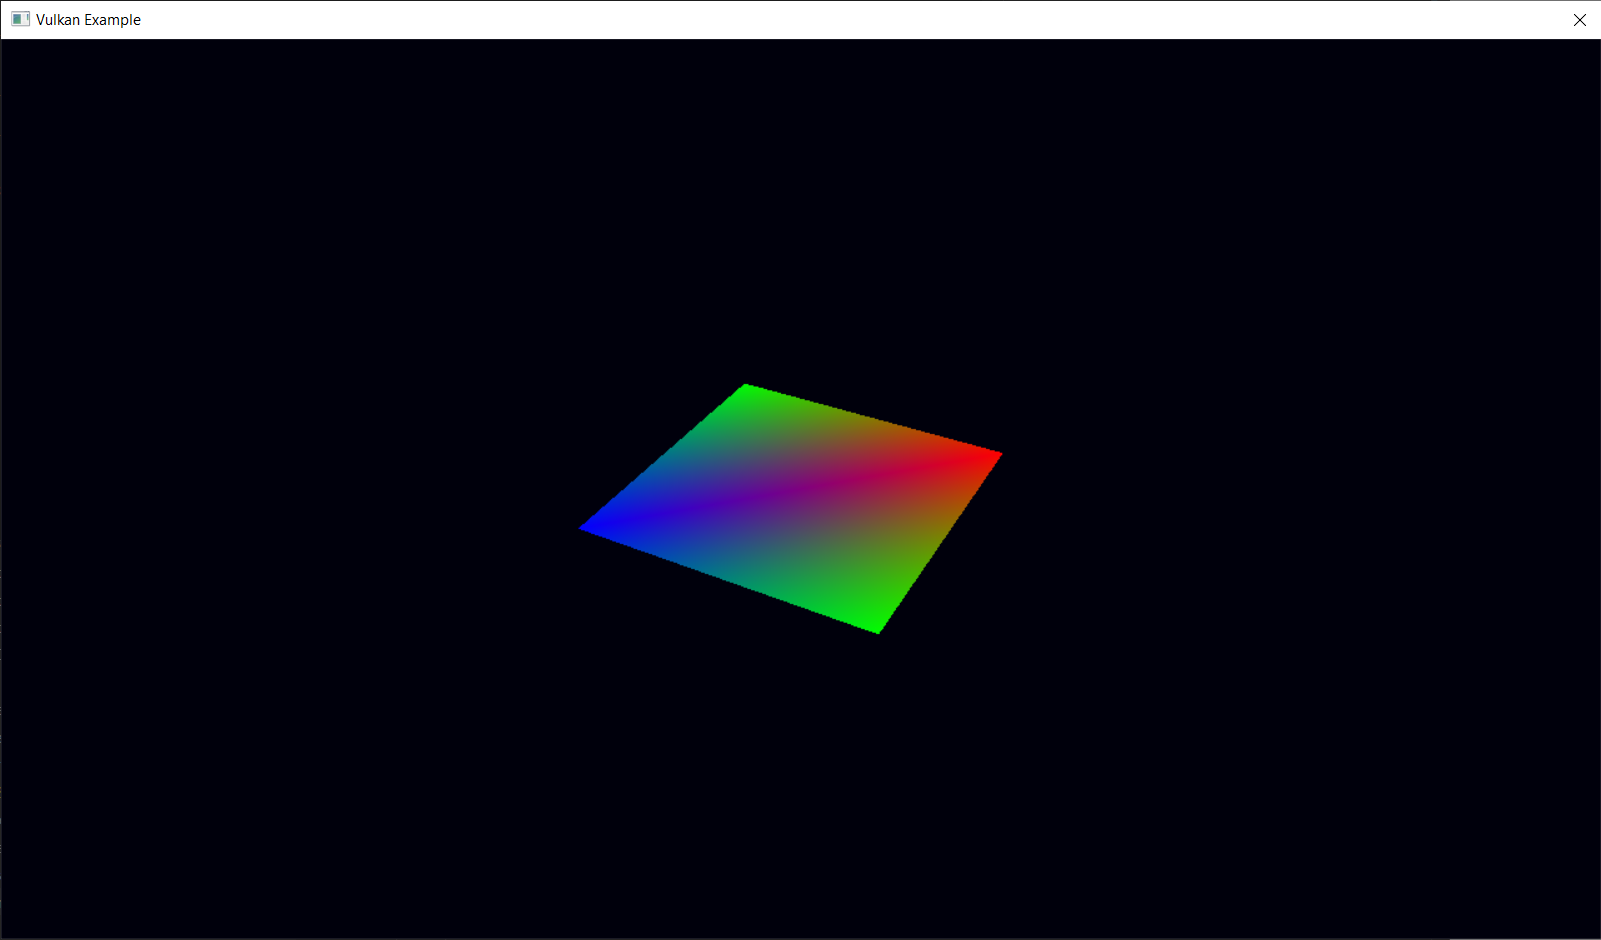
\includegraphics[scale=0.20]{images/ChUniforms/RenderQuad.png}
    \caption{Rendering a quad using a perspective camera}
    \label{fig::RenderQuadUniforms}
\end{figure}

\section{Uniform Data}

In this section we define the uniform data that we use to draw our quad.

\subsection{Uniforms}

In our case, we use three uniforms:
a model matrix,
a view matrix,
and a projection matrix.

\begin{minipage}{\linewidth}{\noindent}
    \lstinputlisting[
        language=C++,
        caption={Data that will be globally available to our shaders},
        label={lst::Uniforms}
        ]{src/ChUniforms/Uniforms.cpp}
\end{minipage}

\subsection{Uniform Buffer Data}

Every frame we update our uniforms as follows.

\begin{minipage}{\linewidth}{\noindent}
    \lstinputlisting[
        language=C++,
        caption={Updating uniforms during the application's main loop},
        label={lst::UpdateUniforms}
        ]{src/ChUniforms/UpdateUniforms.cpp}
\end{minipage}

We use our model matrix to continuously rotate the quad based on the
amount of time since the application has started.
We use our view matrix to represent a camera with position at coordinates
$(2, 2, 2)$, looking at $(0, 0, 0)$ and with $(0, 0, 1)$ as up vector.
We use our projection matrix to define the frustum of our camera.
Here we use a perspective projection with a field of view of $45$ degrees,
an aspect ratio based on the swapchain image, and a near and far planes of
$0.1$ and $10$ respectively.

\subsection{Vertex Shader}

We must update the vertex shader for us to use our uniform data.
In our case, we use a single uniform buffer containing our uniforms.

\begin{minipage}{\linewidth}{\noindent}
    \lstinputlisting[
        language=C++,
        caption={Vertex shader that uses our uniforms},
        label={lst::UniformsVertexShader}
        ]{src/ChUniforms/UniformsVertexShader.vert}
\end{minipage}

In the vertex shader, we transform the vertex position using our matrices.
This is the usual way in which we change vertex data.
Instead of directly modifying vertices, we use one or more matrices
that define the transformation we want.
This computation is very fast because it's executed concurrently on the GPU.

\section{Upload Uniform Data To The GPU}

Uniform data usually changes very frequently, even on a frame by frame basis.
This being the case, every time our uniforms change, we upload them
to the GPU to make the change visible to the shaders that use them.
We use a buffer to upload uniform data to the GPU.
Such buffer is called a uniform buffer.

\subsection{Uniform Buffer Layout}

Before creating a uniform buffer, we declare its layout.
In our case, since we have three uniforms, we pack them
together inside a uniform buffer.

\begin{minipage}{\linewidth}{\noindent}
    \lstinputlisting[
        language=C++,
        caption={Uniform buffer definition},
        label={lst::UBO}
        ]{src/ChUniforms/UBO.cpp}
\end{minipage}

\subsection{Uniform Buffer Creation}

We use the \texttt{VK\_BUFFER\_USAGE\_UNIFORM\_BUFFER\_BIT} flag because
our buffer will be used by the GPU as a uniform buffer.

We use the \texttt{VK\_MEMORY\_PROPERTY\_HOST\_VISIBLE\_BIT} flag because
we want our buffer to be host visible.
This is due to the fact that we upload our uniforms to the uniform buffer
every frame.

We use the \texttt{VK\_MEMORY\_PROPERTY\_HOST\_COHERENT\_BIT} flag because
we don't want to manually flush our buffer memory.

\begin{minipage}{\linewidth}{\noindent}
    \lstinputlisting[
        language=C++,
        caption={Uniform buffer creation},
        label={lst::UBOCreation}
        ]{src/ChUniforms/UBOCreation.cpp}
\end{minipage}

\subsubsection{Cleanup}

We use \texttt{vkFreeMemory} and \texttt{vkDestroyBuffer} to clean up a
uniform buffer.

\subsection{Upload Uniform Data}

We upload our uniform data simply by writing it into our uniform buffer.

\begin{minipage}{\linewidth}{\noindent}
    \lstinputlisting[
        language=C++,
        caption={Upload uniforms to the uniform buffer},
        label={lst::UploadUniforms}
        ]{src/ChUniforms/UploadUniforms.cpp}
\end{minipage}

\subsection{Uniform Buffer Data Alignment}

Vulkan expects the data in our uniform buffer to be aligned in memory
in a specific way.
You can find the full list of alignment requirements in the
\href{https://www.khronos.org/registry/vulkan/specs/1.3-extensions/html/chap15.html#interfaces-resources-layout}{Vulkan specification}.
Here follows a brief list of the most important requirements.

\begin{itemize}
\item Scalars have to be aligned by $N$ (for example, $4$ bytes for \texttt{f32} values)
\item A \texttt{vec2} must be aligned by $2N$
\item A \texttt{vec3} or \texttt{vec4} must be aligned by $4N$
\item A structure must be aligned by the base alignment
of its members rounded up to a multiple of $16$
\item A \texttt{mat4} matrix must have the same alignment as a \texttt{vec4}
\end{itemize}

\section{Update Pipeline Layout}

We must inform our pipeline that we are using one or more uniforms.
To do this we update our pipeline layout.

\subsection{VkPipelineLayout}

A pipeline layout can be seen as an interface between shader stages
and shader resources as it takes these groups of resources, describes how
they are gathered, and provides them to the pipeline.

\begin{minipage}{\linewidth}{\noindent}
    \lstinputlisting[
        language=C++,
        caption={Update pipeline layout creation},
        label={lst::UpdatePipelineLayoutCreation}
        ]{src/ChUniforms/UpdatePipelineLayoutCreation.cpp}
\end{minipage}

\subsection{Descriptor Set Layout}

We use a \texttt{VkDescriptorSetLayout} object to tell the number and the types
of global resources that are available to our pipeline shaders.

\begin{minipage}{\linewidth}{\noindent}
    \lstinputlisting[
        language=C++,
        caption={Describe pipeline global resources},
        label={lst::CreateDescriptorSteLayout}
        ]{src/ChUniforms/CreateDescriptorSteLayout.cpp}
\end{minipage}

\subsubsection{VkDescriptorSetLayoutCreateInfo}

We use a \texttt{VkDescriptorSetLayoutCreateInfo} struct to configure the
descriptor set layout we are about to create.

\begin{minipage}{\linewidth}{\noindent}
    \lstinputlisting[
        language=C++,
        caption={Descriptor set layout configuration},
        label={lst::VkDescriptorSetLayoutCreateInfo}
        ]{src/ChUniforms/VkDescriptorSetLayoutCreateInfo.cpp}
\end{minipage}

\subsubsection{Descriptor Set Layout Bindings}

We use a \texttt{VkDescriptorSetLayoutBinding} to describe, for a given type,
how many resources are globally available to our pipeline.
In our application we use only one uniform buffer accessed from the vertex shader.

\begin{minipage}{\linewidth}{\noindent}
    \lstinputlisting[
        language=C++,
        caption={Descriptor set layout bindings},
        label={lst::DescriptorSetLayoutBindings}
        ]{src/ChUniforms/DescriptorSetLayoutBindings.cpp}
\end{minipage}

\texttt{binding} is the binding number of this entry and corresponds to
a resource of the same binding number in the shader stages.
We have seen this binding number in our vertex shader when we wrote
\texttt{layout(set = 0, binding = 0) uniform UBO} to access the uniform buffer.
\texttt{descriptorType} is a \texttt{VkDescriptorType} specifying which type of
resource descriptors are used for this binding.
\texttt{descriptorCount} is the number of resources contained in the binding.
\texttt{stageFlags} is a bitmask of \texttt{VkShaderStageFlagBits} specifying which
pipeline shader stages can access a resource for this binding
\subsubsection{Cleanup}

We use \texttt{vkDestroyDescriptorSetLayout} do destroy a descriptor
set layout.

\section{Descriptor Set}

A descriptor set is an object that contains all the physical resources that
are globally available to a set of pipeline shader stages.
We allocate a descriptor set from a descriptor pool.
Then we populate the descriptor set with one or more resources.

\subsection{Descriptor Set Allocation}

We allocate a descriptor set with \texttt{vkAllocateDescriptorSets}.

\begin{minipage}{\linewidth}{\noindent}
    \lstinputlisting[
        language=C++,
        caption={Allocate a descriptor set},
        label={lst::AllocateDescriptorSet}
        ]{src/ChUniforms/AllocateDescriptorSet.cpp}
\end{minipage}

\subsection{VkDescriptorSetAllocateInfo}

We use a \texttt{VkDescriptorSetAllocateInfo} struct to configure the descriptor
set we are about to create.

\begin{minipage}{\linewidth}{\noindent}
    \lstinputlisting[
        language=C++,
        caption={Configure descriptor set},
        label={lst::VkDescriptorSetAllocateInfo}
        ]{src/ChUniforms/VkDescriptorSetAllocateInfo.cpp}
\end{minipage}

\texttt{descriptorPool} is the pool which the sets will be allocated from.
\texttt{descriptorSetCount} determines the number of descriptor sets to be
allocated from the pool.
\texttt{pSetLayouts} is a pointer to an array of descriptor set layouts,
with each member specifying how the corresponding descriptor set is allocated.

\section{Descriptor Pool}

A descriptor set must be allocated from a descriptor pool.
Thus, we must create a descriptor pool before allocating a descriptor set.

\begin{minipage}{\linewidth}{\noindent}
    \lstinputlisting[
        language=C++,
        caption={Create descriptor pool},
        label={lst::CreateDescriptorPool}
        ]{src/ChUniforms/CreateDescriptorPool.cpp}
\end{minipage}

\subsection{VkDescriptorPoolCreateInfo}

We use a \texttt{VkDescriptorPoolCreateInfo} struct to configure the descriptor
pool we are about to create.
In our case, since we use only one uniform buffer, we create a descriptor pool
from which we can allocate only one descriptor set with one uniform buffer resource.

\begin{minipage}{\linewidth}{\noindent}
    \lstinputlisting[
        language=C++,
        caption={Configure descriptor poll creation},
        label={lst::VkDescriptorPoolCreateInfo}
        ]{src/ChUniforms/VkDescriptorPoolCreateInfo.cpp}
\end{minipage}

\texttt{maxSets} is the maximum number of descriptor sets that can be allocated
from the pool.
\texttt{pPoolSizes} is a pointer to an array of \texttt{VkDescriptorPoolSize}
structures, each containing a descriptor type and the number of resources
of that type that will be allocated in total from the pool.

\subsection{Populate Descriptor Set}

Once we have allocated a descriptor set, we have to populate it with resources.
This means writing into the descriptor set.
We use \texttt{vkUpdateDescriptorSets} for this task.

\begin{minipage}{\linewidth}{\noindent}
    \lstinputlisting[
        language=C++,
        caption={Populate descriptor set},
        label={lst::UpdateDescriptorSets}
        ]{src/ChUniforms/UpdateDescriptorSets.cpp}
\end{minipage}

\subsection{VkWriteDescriptorSet}

We use a \texttt{VkWriteDescriptorSet} struct to configure the descriptor
write operations that we are about to execute.
Here we are telling our descriptor set to use our uniform buffer as a
uniform buffer resource.

\begin{minipage}{\linewidth}{\noindent}
    \lstinputlisting[
        language=C++,
        caption={Descriptor set write},
        label={lst::VkWriteDescriptorSet}
        ]{src/ChUniforms/VkWriteDescriptorSet.cpp}
\end{minipage}

\subsection{Cleanup}

We use \texttt{vkDestroyDescriptorPool} to destroy a descriptor pool.
All descriptor sets allocated from the pool will be automatically
freed when the pool is destroyed.

\section{Draw Using Our Uniform Data}

The only thing missing now is to tell Vulkan to use our uniforms during rendering.
To accomplish this, we tell Vulkan to use the resources that are inside
our descriptor set for rendering.
We do this during our command buffer recording.

\begin{minipage}{\linewidth}{\noindent}
    \lstinputlisting[
        language=C++,
        caption={Draw quad using our uniform data},
        label={lst::DrawWithUniformBuffer}
        ]{src/ChUniforms/DrawWithUniformBuffer.cpp}
\end{minipage}
